\documentclass[11pt]{beamer}
\usetheme{Berlin}
\usecolortheme{beaver}
\usepackage[utf8]{inputenc}
\usepackage[english]{babel}
\usepackage{amsmath}
\usepackage{amsfonts}
\usepackage{amssymb}
\author{Nicolas Kobel \\Stephane Donnet \\Loïc Haas \\João Miguel Pedrosa Domingues}
\title{Transfusion D'Étérnité}
%\setbeamercovered{transparent} 
%\setbeamertemplate{navigation symbols}{} 
%\logo{img/logo.png} 
%\institute{} 
%\date{} 
%\subject{} 

%\usebackgroundtemplate%
%{%
%    
\includegraphics[height=\paperheight]{img/logo.png}%
%}
\begin{document}

\begin{frame}
\titlepage
\end{frame}

\begin{frame}
\tableofcontents
\end{frame}

\section{L'entreprise}
\begin{frame}
\frametitle{Qui Sommes Nous}
\begin{itemize}[<+->]
\item Janvier 2015 : Première Idée
\item Août 2015 : Première Production
\item Septembre à Novembre 2015 : Première Commércialisation
\item Futur : Formalisation de l'entreprise
\end{itemize}
\end{frame}
\section{Histoire de l'Hypocras}
\begin{frame}{Histoire de l'hypocras}
     \begin{columns}[c] % contents are top vertically aligned
     \begin{column}[c]{5cm} % each column can also be its own environment
     \begin{itemize}[<+->]
     \item Antiquité
     % les premières recettes connues datent de pline l'ancien, ancien chroniqueur Romain (Ier siecle ap J-C.
     \item Moyen Âge
     % Aux moyen age les épices aidaient à masquer le goût de vins de mauvaise qualité
     \item Modernité
     % Depuis le XVIIIe siècle l'hypocras a disparu de la vie de tout les jours.
     % Petites productions en france, utilisé dans la cuisine locale
     \end{itemize}
     \end{column}
     \begin{column}[c]{5cm} % alternative top-align that's better for graphics
          \includegraphics<1>[height=3cm]{img/pline.jpeg}
          \includegraphics<2>[width=\textwidth]{img/histoire_moyenage.jpg}
          \includegraphics<3>[width=\textwidth]{img/ypocras_recette.jpg}
     \end{column}
     \end{columns}

\end{frame}

\section{Actualité de l'Hypocras}
\begin{frame}{Une viellerie ? Mais NON!}
     \begin{columns}[c] % contents are top vertically aligned
     \begin{column}[c]{5cm} % each column can also be its own environment
     \begin{itemize}[<+->]
     \item Bâle
     % IMG -> la aadringgede (pronontiacion adrinquédé) tradition baloise ou une fontaine dispense de
     % l'hypocras pendant le jour de l'An.
     \item Bars Spécialisés
     % Certains bars spécialisés vendent de l'hypocras, par expemle le banshee's lodge à Fribourg
     \item Reconstitutions Médiévales
     % Les festivals de reconstitutions médiévales ainsi que les JDR GN ont souvent des stands de distribution de boisson ou on y trouve hypocras et hydromel 
     \end{itemize}
     \end{column}
     \begin{column}[c]{5cm} % alternative top-align that's better for graphics
          \includegraphics<1>[width=\textwidth]{img/aadringgede.jpg}
          \includegraphics<2>[width=\textwidth]{img/bansheeslodge2.jpg}
          \includegraphics<3>[width=\textwidth]{img/larp.jpg}
     \end{column}
     \end{columns}

\end{frame}
\section{Le Produit}
\begin{frame}{Hypocras Transfusion d'Étérnité}
\begin{center}

\includegraphics<1>[height=\textheight]{img/logo.png}
\includegraphics<2>[height=\textheight]{img/boutteilles.jpg}
\end{center}
% Photos du produit Logo
% Dates clés production
\end{frame}
\begin{frame}{Un produit local et bio}
     \begin{columns}[c] % contents are top vertically aligned
     \begin{column}[c]{5cm} % each column can also be its own environment
     \begin{itemize}[<+->]
     \item Vins de la côte
     % TdE est en négociation avec des producteurs de la région de vevey
     \item Miel Gruyèrien
     % Des amis apiculteurs fournissent TdE en miel
     \item Accentuation sur le Bio
     % Afin d'offrir la meilleure qualité nous misons sur des matières premières de bonne qualité
     % avec un accent sur les produits bio
     \end{itemize}
     \end{column}
     \begin{column}[c]{5cm} % alternative top-align that's better for graphics
          \includegraphics<1>[width=\textwidth]{img/vignes.jpg}
          \includegraphics<2>[width=\textwidth]{img/apiculteur.png}
          \includegraphics<3>[width=\textwidth]{img/Bio_Knospe.jpg}
     \end{column}
     \end{columns}

\end{frame}
\section{Fabrication}
\begin{frame}{Une fabrication moderne}
     \begin{columns}[c] % contents are top vertically aligned
     \begin{column}[c]{5cm} % each column can also be its own environment
     \begin{itemize}[<+->]
     \item Fabrication Main
     % Les premières séries tests ont étés réalisés à la main
     \item Machines imaginées
     % Dans le cadre du cours nous avons imaginé une machine qui nous permetterais d'automatiser le processus
     \item Vers des grandes quantités
     % Les quantités prévues se trouvent dans la 100-aine de litres par mois,
     % si TdE devient un projet à plein temps une méchanisation doit être prévue.
     \end{itemize}
     \end{column}
     \begin{column}[c]{5cm} % alternative top-align that's better for graphics
          \includegraphics<1>[width=\textwidth]{img/fabrication_ancienne.jpg}
          %TODO sketch
          \includegraphics<3>[width=\textwidth]{img/gabs.jpg}
     \end{column}
     \end{columns}
\end{frame}
\section{Distribution}
\begin{frame}{Une distribution Révolutionnaire}
  \begin{columns}[c] % contents are top vertically aligned
     \begin{column}[c]{5cm} % each column can also be its own environment
     \begin{itemize}[<+->]
     \item Commande Internet
     % 30\% de la production est déstinée à la vente directe
     \item Magasins spécialisés
     % La première production a été commércialisé grace à la mise en bière à Lausanne
     \item Bars
     % Nous avons fait déguster notre produit à plusieurs bars notamment le pi bar à lausanne qui
     % s'est montré interéssé 
     \end{itemize}
     \end{column}
     \begin{column}[c]{5cm} % alternative top-align that's better for graphics
          \includegraphics<1>[width=\textwidth]{img/commandeInternet.jpg}
          \includegraphics<2>[width=\textwidth]{img/mise_en_biere.jpg}
          \includegraphics<3>[width=\textwidth]{img/pibar.jpg}
     \end{column}
   \end{columns}
\end{frame}

\section{Marketing}
\begin{frame}{Du Marketing de Proximité}
  \begin{columns}[c] % contents are top vertically aligned
     \begin{column}[c]{5cm} % each column can also be its own environment
     \begin{itemize}[<+->]
     \item Vers le public cible
     % Notre public cible est assez restraint et se réunit régulièrement, c'est à ces occasions (GN,
     % reconstitutions) que nous pouvons le rencotrer
     \item Dégustations
     % La découverte de l'hypocras peut se faire par des dégustations organisées dans des bars ou lors
     % de conventions de JDR / médievalistes
     \item Éducation
     % Nous voulons informer nos clients de l'histoire du produit. Des flyers explicatifs se trouvent
     % aux points de vente et lors de nos actions publicitaires.
     \item Réseaux sociaux
     % La plus-part du marketing passif se fera sur des réseaux sociaux en ligne, par le biais d'une
     % notemment par une page facebook
     % Des promotions exceptionnelles ainsi que des invitations aux conventions ou nous apparaissont 
     % seront envoyées aux clients inscrits dans notre base de données
     \end{itemize}
     \end{column}
     \begin{column}[c]{5cm} % alternative top-align that's better for graphics
          \includegraphics<1>[width=\textwidth]{img/banshees_2.jpg}
          \includegraphics<2>[width=\textwidth]{img/conv.jpg}
          \includegraphics<3->[width=\textwidth]{img/flyer.jpg}
     \end{column}
   \end{columns}
% plus de photos de bar
% plus de photos de GN
% plus de photos de Conv
\end{frame}
\section{Conclusion}
\begin{frame}{En 10 mots}
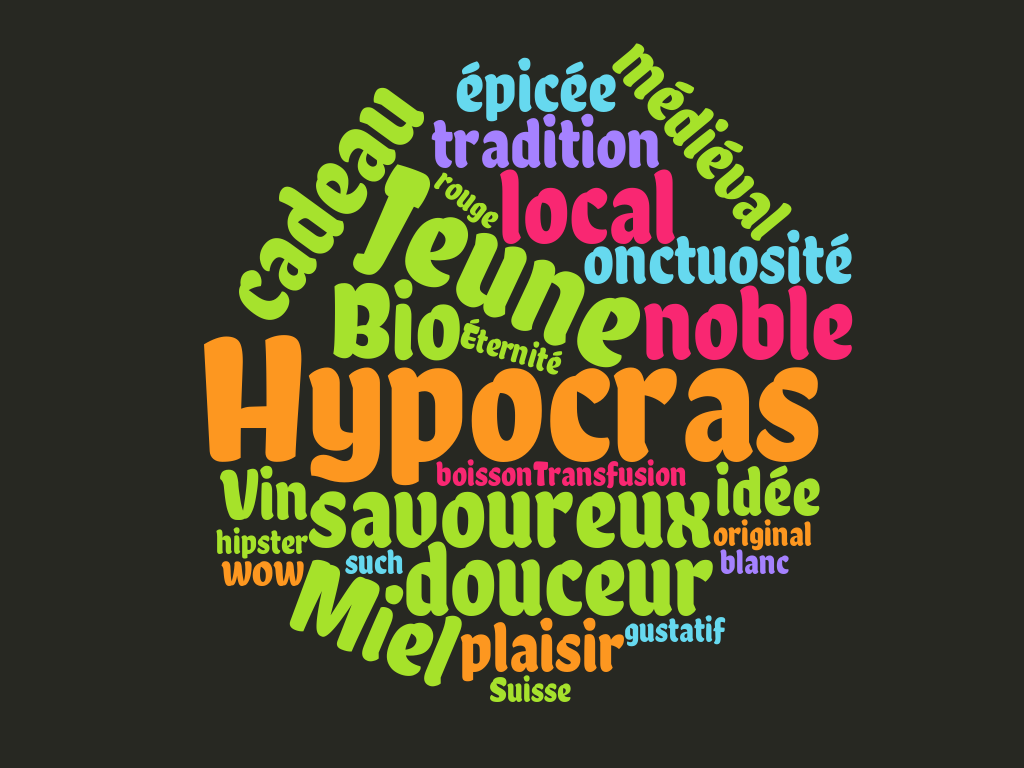
\includegraphics[height=\textheight]{img/wordcloud_round.png}
\end{frame}
\end{document}